\chapter{Implementierung}
	Aus den oben beschrieben Überlegungen und dem in \cref{fig:flowchart} gezeigten grundlegenden Programmablauf folgt die nachfolgend beschriebene Implementierung in Software.
	Zeilen 7-9 der \textit{main.cpp} importieren neben der online verfügbaren Bibliothek \texttt{mouse.h}, die die nötigen Funktionalitäten zur Steuerung der Maus des Host-Computers zur Verfügung stellt, die beiden Header-files \texttt{defines.h} und \texttt{helper\_functions.h} (siehe \crefrange{lst:main cpp}{lst:defines h}).
	\texttt{defines.h} beinhaltet Konstanten in Form von Compilerdefinitionen, die zur Laufzeit nicht geändert werden.
	In \texttt{helper\text\_funtions.h} bzw. \texttt{helper\text\_functions.cpp} sind die direkt mit dem Touchscreen in Zusammenhang stehenden Funktionen ausgegliedert.\par\medskip

	Zeilen 21-23 der \texttt{main.cpp} initialisieren drei globale Variablen -- für jede Achsrichtung ein Array der Länge \texttt{OVERSAMPLING} (siehe \texttt{defines.h}) und ein Pointer, die im weiteren Verlauf zur Auswertung benötigt werden.

	\section{Vorbereitung der MCU}
		Um mögliche Fehlerquellen etwa durch \textit{cross-talking} zwischen GPIOs und der ADC auszuschließen, werden wie in \cite{MicrochipTechnologyInc.ATmega32U4.Datasheet.2016} auf Seite 71 beschrieben alle ungenutzten Pins in einen definierten Zustand -- hier als \textit{Input} mit aktiviertem \textit{Pull-Up} -- versetzt.
		Als Schnittstelle zum Touchscreen kommen nur Pins an Port F zum Einsatz welche vorbereitend ebenfalls als Input, allerdings ohne Pull-Up konfiguriert werden.\par\medskip

		Die internen ADC verwenden einen eigenen Timer der durch Setzen der Bits \texttt{ADPSx} im \texttt{ADCSRA}-Register konfiguriert wird.
		Diese bestimmen den Prescaler, der die CPU-Clock auf die gewünschte ADC-Frequenz herunter teilt.
		Um die volle Auflösung der ADC sicher ausnutzen zu können, darf die Frequenz des ADC-Timers gemäß Datenblatt \SI{200}{\kilo\hertz} nicht überschreiten.
		\begin{figure}[h]
			\centering
			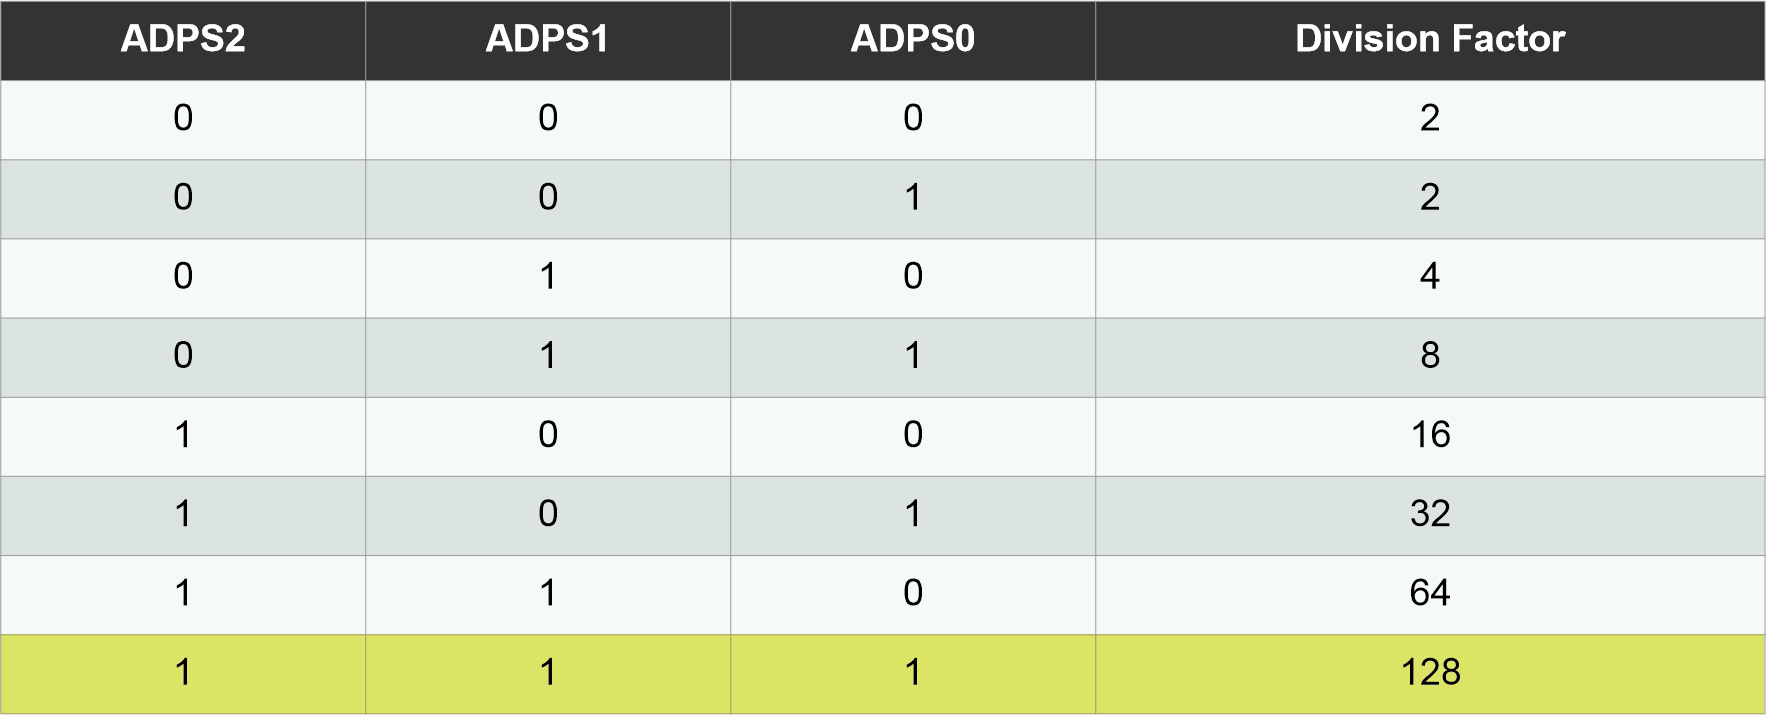
\includegraphics[width=.9\textwidth]{fig/raster/ADC-Timer_Config.png}
			\caption[Auszug aus dem Datenblatt zu den relevanten Bits des Registers \texttt{ADCSRA}]{Auszug aus dem Datenblatt zu den relevanten Bits des Registers \texttt{ADCSRA} (Seite 316 \cite{MicrochipTechnologyInc.ATmega32U4.Datasheet.2016}).}
			\label{fig:adc timer konfig}
		\end{figure}
		Die möglichen Werte der Prescaler des ADC-Timers sind in \cref{fig:adc timer konfig} gezeigt.
		Mit der gelb hinterlegten Konfiguration errechnet sich die maximale ADC-Frequenz unter Beibehalt einer Auflösung von 10Bit zu
		\begin{equation}
			f_{ADC} = \frac{\SI{16}{\mega\hertz}}{128} = \SI{125}{\kilo\hertz}
			\label{eq:adc timer}
		\end{equation}
		was sich zu einer Periodendauer für einen Taktzyklus von \SI{8}{\micro\second} übersetzt.
		Weiter geht aus dem Datenblatt hervor, dass die Samplingdauer des ADC 1,5 Zyklen und die Konvertierungsdauer 13 Zyklen des ADC-Timers benötigt.
		Mit dem gewählten Prescaler ergibt sich so die benötigte Mindestdauer für eine Messung von
		\begin{align}
			t_{messung} &= t_{Sample} + t_{Hold} = \frac{n_{Sample}}{f_{ADC}} + \frac{n_{Hold}}{f_{ADC}} \nonumber \\
						&= \SI{14}{\micro\second} + \SI{102}{\micro\second} = \SI{116}{\micro\second}
			\label{eq:adc messdauer}
		\end{align}

		Dem Datenblatt des verwendeten Touchscreens ist zu entnehmen, dass mit einer maximalen Eingangsimpedanz zum ADC von \SI{850}{\ohm} (x-Richtung) zu rechnen ist \cite{FUJITSU.touchscreen.datasheet}.
		\Cref{fig:analog input circuitry} zeigt die interne Eingangsverschaltung der ADC der verwendeten MCU. Die Kapazität \(C_{S/H}\) gilt es in der Zeit \(t_{Sample}\) auf einen Wert \(\frac{U_0}{2} \pm \frac{1}{2}LSB\) zu laden.

		\begin{gather}
			\frac{U_0}{2} - \frac{1}{2}LSB = U_0 \left( 1 - e^{-\frac{t_{Sample}}{RC}} \right) \nonumber \\
			\Leftrightarrow \nonumber \\
			t_{Sample} = -ln\left( \frac{1LSB}{2U_0} + \frac{1}{2}\right) \cdot RC
			\label{eq:samplingzeit}
		\end{gather}

		Mit Werten für \(R\), \(C_{S/H}\), \(U_0\) von \SI{850}{\ohm}, \SI{14}{\pico\farad} und \SI{5}{\volt} und \(\frac{1}{2}LSB = \frac{U_0}{2 \cdot 2^{10}}\) ergibt sich eine benötigte Samplingdauer von
		\begin{align}
			t_{Sample}	&= -ln\left( \frac{1}{2\cdot 2^{10}} + \frac{1}{2}\right) \cdot RC \nonumber \\
						&= -ln\left( \frac{1}{2\cdot 2^{10}} + \frac{1}{2}\right) \cdot \SI{850}{\ohm} \cdot \SI{14}{\pico\farad} \nonumber \\
						&= \SI{8,23}{\nano\second}
			\label{eq:samplingzeit gerechnet}
		\end{align}
		was sehr gut im Rahmen der gewählten ADC-Timerfrequenz liegt.
		Ebenso deckt es sich gut mit der Angabe des Datenblattes, bei Eingangsimpedanzen unterhalb von \SI{10}{\kilo\ohm} seien Samplingzeiten vernachlässigbar.
		\begin{figure}[h]
			\centering
			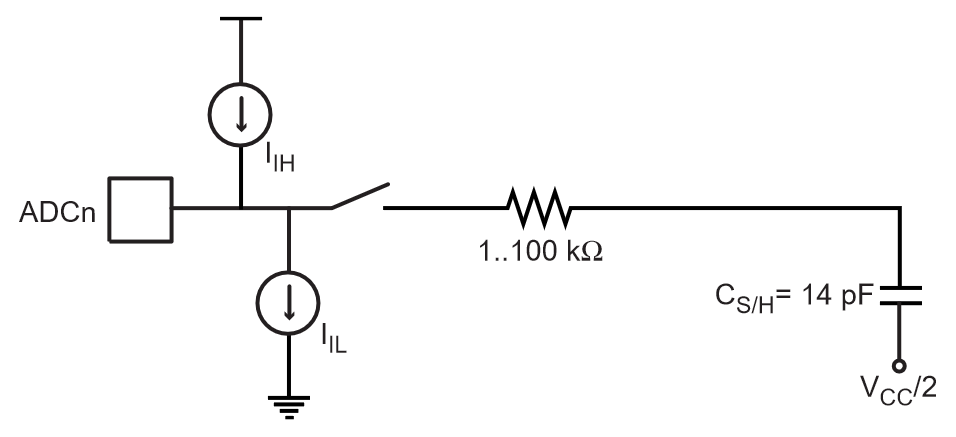
\includegraphics[width=.8\textwidth]{fig/raster/adc-input-circuit.png}
			\caption[Interne Eingangsverschaltung der ADC]{Interne Eingangsverschaltung der ADC wie im Datenblatt gezeigt. Die Kapazität \(C_{S/H}\) ist hier der \textit{Sample and Hold}-Kondensator.}
			\label{fig:analog input circuitry}
		\end{figure}

		Zuletzt wird der externe Interrupt \texttt{INT0} an Pin PD0 im Register \texttt{EIMSK} durch Setzen des Bits \texttt{INT0} aktiviert und im Register \texttt{EICRA} so konfiguriert, dass er auf steigende, wie fallende Flanken reagiert.
		Die Firmware soll in der Lage sein durch einen externen Schalter -- in \cref{fig:aufbau} Position 4 -- zwischen der Ausgabe von Koordinatenpaaren über die serielle Schnittstelle und der Steuerung der Maus des angeschlossenen PCs umschalten zu können. Zusätzlich wird die auf dem \textsc{Arduino}-Board befindliche LED als visueller Indikator des aktuellen Betriebsmodus genutzt.
		Das An- und Abschalten der LED erfolgt in der entsprechenden Interrupt-Serviceroutine.\par

		Zuletzt werden mit den befehlen
		\begin{lstlisting}[language=C++]
			Serial.begin(115200);
			Mouse.begin();
		\end{lstlisting}
		die oben erwähnte serielle Schnittstelle, sowie die Emulation der Maus initialisiert.

	\section{Hauptschleife und Unterfunktionen}
		Im Programmablauf werden in drei verschiedenen Situationen Konversionen der ADC benötigt.
		Während es sich hier durchaus um verschiedene physische ADC handeln kann, ist der grundlegende Ablauf wie etwa das Auslesen des Wandlungsergebnisses aus den entsprechenden Registern stets gleich.
		Diese sich wiederholende Routine leistet die Funktion \texttt{getADC()} in den Zeilen 35 bis 45 der \texttt{helper\_functions.cpp}.
		In zwei Schritten wird hier durch Setzen der Bits \texttt{ADSC} und \texttt{ADEN} des Registers \texttt{ADCSRA} die ADC-Peripherie aktiviert und eine Konvertierung am zuvor verbundenen ADC-Eingang gestartet.
		Die folgende Schleife überprüft periodisch den Zustand des Bits \texttt{ADSC}, welches nach Beendigung einer Konvertierung vom System automatisch auf 0 zurückgesetzt wird.\par
		Das Wandlungsergebnis befindet sich in den 8 Bit des Registers \texttt{ADCL} und den beiden niederwertigsten Bits des Registers \texttt{ADCH}.
		Da jede weitere Operation, die eines der beiden Register schreibend manipulieren würde -- wie etwa eine nachfolgende Konvertierung durch einen beliebigen anderen ADC -- den Inhalt der Register und damit das Wandlungsergebnis unbrauchbar machen würde, wird unmittelbar nach Verlassen der Schleife lesend auf die beiden Register zugegriffen.
		Sobald lesend auf das niederwertige Register \texttt{ADCL} zugegriffen wird, wird der Inhalt des höherwertigen Registers gegen Schreibzugriffe geschützt, bis auch auf jenes lesend zugegriffen wurde.
		Umgesetzt wird dies durch Erstellen einer 16Bit breiten lokalen Variable \texttt{val}, in deren niederwertigeren 8 Bit der Inhalt von \texttt{ADCL} geschrieben wird.
		Anschließend wird \texttt{val}, um 8 Bit verschoben, mit dem Inhalt von \texttt{ADCH} oder-verknüpft manipuliert.

		Um eine Messung zu verhindern, während der Touchscreen gerade nicht berührt wird, werden innerhalb der Funktion \texttt{isFingered()} die Pins \texttt{PF4}-\texttt{PF7} wie in \cref{fig:fingered} konfiguriert (vgl. \cref{fig:schaltbild}).
		\begin{figure}[h]
			\centering
			\includesvg[width=.6\textwidth]{fig/schematics/sch_fingering}
			\caption{Pinkonfigurationen und Schaltbild zur Überprüfung einer validen Berührung.}
			\label{fig:fingered}
		\end{figure}
		Wie \cref{fig:schaltbild} zu entnehmen sind hier Pin \texttt{PF7} als Ausgang und LOW und PF7 als Eingang mit aktiviertem Pull-Up konfiguriert während Pins \texttt{PF5} und \texttt{PF6} als digitale Eingänge mit hoher Eingangsimpedanz konfiguriert sind und so für die Anwendung als inexistent betrachtet werden können.
		Über den Pull-Up Widerstand auf \(U_{vcc}\) gelegt liefert der ADC in dieser Konfiguration stets einen Wert von 1023 was dem Maximum seines Messbereichs entspricht.
		Da bei einer validen Berührung des Touchscreens selbst im ungünstigsten Fall den Eingang des ADC über einen Serienwiderstand von \(\SI{850}{\ohm} + \SI{600}{\ohm}\) effektiv auf Masse legt, wird das Wandlungsergebnis nahe am unteren Wertebereich liegen und ermöglicht so eine sichere Detektion einer Berührung.
		Es folgt, dass der absolute Wert des Wandlungsergebnisses hier nicht von weiterem Interesse ist und lediglich gegen einen vordefinierten, empirisch ermittelten Wert verglichen wird.\par\medskip

		Im Falle einer detektierten Berührung wird die Funktion \texttt{readX()} aufgerufen innerhalb derer Pins \texttt{PF7} und \texttt{PF6} als Ausgänge und HIGH bzw. LOW gesetzt werden.
		Nachdem Pin \texttt{PF5} auf den Eingang des ADC geschaltet wurde, wird wiederum \texttt{getADC()} aufgerufen was eine Messung wie oben beschrieben auslöst.
		Von der Funktion wird anschließend das Wandlungsergebnis zur weiteren Verarbeitung zurückgegeben.
		\begin{figure}[h]
			\centering
			\includesvg[width=.6\textwidth]{fig/schematics/sch_read_x}
			\caption{Schaltbild zur Messung der Position entlang der horizontalen Achse des Touchscreens.}
			\label{fig:readX schaltbild}
		\end{figure}
		Die beiden Widerstände \(R_{xh}\) und \(R_{xl}\) bilden hier einen Spannungsteiler dessen Verhältnis von der Druckposition entlang der horizontalen des Touchscreens abhängig ist.
		\(R_{yh}\) trägt hier zur Eingangsimpedanz zum ADC nach \cref{eq:samplingzeit} bei und kann auch im ungünstigsten Fall -- er ist von der vertikalen Druckposition abhängig -- vernachlässigt werden.\par
		Ist die Messung abgeschlossen und wird durch ein abermaliges aufrufen von \texttt{getADC()} noch eine Berührung detektiert, wird \texttt{readY()} aufgerufen.
		Die Messung findet in leicht abgeänderter Form wie in \cref{fig:readY schaltbild} gezeigt statt, der grundlegende Prozess ist aber unverändert und soll hier nicht wiederholt werden.
		\begin{figure}[h]
			\centering
			\includesvg[width=.6\textwidth]{fig/schematics/sch_read_y}
			\caption{Schaltbild zur Messung der Position entlang der horizontalen Achse des Touchscreens.}
			\label{fig:readY schaltbild}
		\end{figure}

		\subsection{Filterung}
			Um gröbere Ausreißer der Messungen zu unterdrücken wird ein Median-Filter verwendet.
			Nachdem eine Anzahl Messungen für jede Achse durchgeführt wurde liegen zwei Arrays der Länge \texttt{OVERSAMPLING} vor.
			Sei \texttt{OVERSAMPLING} ein ganzzahliger Wert \(n\), so werden ausgehend vom Wert an der Stelle \(\lfloor \frac{n}{2}\rfloor\) des jeweiligen Arrays alle Werte \(i\) verworfen, die die Bedingung
			\begin{equation}
				Wert_{\lfloor \frac{n}{2}\rfloor} - CLAMP \leq i \leq Wert_{\lfloor \frac{n}{2}\rfloor} + CLAMP
			\end{equation}
			nicht erfüllen.\par
			Die Umsetzung findet in der Funktion \texttt{doSomeMedianFiltering()} statt.
			Neben dem Array mit den Wandlungsergebnissen müssen der Funktion als obligatorische Argumente die Länge des Arrays und der (obere und untere) Schwellwert der Filterung übergeben werden.
			\texttt{CLAMP} ist hier ebenfalls ein empirisch gefundener Wert und wurde in der Implementierung auf den Wert 2 gesetzt (siehe \texttt{defines.h}).
			Aus den übrigen Werten wird das arithmetische Mittel gebildet und als Ausgabewert zurückgegeben.
			% Dies wird beispielhaft in \cref{fig:medianfilterdarstellung} gezeigt.
			% \begin{figure}[h]
			% 	\centering
			% 	\includesvg[inkscapelatex=false, width=.3\textwidth]{fig/medianfilter}
			% 	\caption{Vereinfachte Darstellung des verwendeten Medianfilters.}
			% 	\label{fig:medianfilterdarstellung}
			% \end{figure}
		\subsection{Betriebsmodi}\label{sec:betriebsmodi}
			Ist der externe Schalter geöffnet, so werden die gefilterten Wertepaare \(w \in W\) auf eine Wertemenge \(s \in S\) abgebildet.
			Die Menge \(W\) ist der Wertebereich, den die Wandlungsergbnisse im Rahmen des sensitiven Bereichs des Touchscreens je Raumrichtung annehmen können und müssen im Vorfeld experimentell gefunden werden.
			Für \(S\) gilt
			\begin{equation}
				S=
				\begin{cases}
					0 \leq s \leq B \qquad \text{für } x\\
					0 \leq s \leq H \qquad \text{für } y
				\end{cases}
			\end{equation}
			mit der Abbildungsvorschrift
			% über \(0 \leq s \leq WIDTH\) für die horizontale und \(0 \leq s \leq HEIGHT\) für die vertikale Richtung oder über \(-MOUSE_SPEED \leq s \leq MOUSE_SPEED\).
			% Die Abbildungsvorschrift lässt sich allgemein wie in \cref{eq:mapping} schreiben.
			% Diese sind durch \texttt{XMIN} und \texttt{XMAX} bzw. \texttt{YMIN} und \texttt{YMAX} vordefiniert und wurden durch
			\begin{equation}
				s(w) = \frac{w - w_{min}}{w_{max} - w_{min}} \cdot (s_{max} - s_{min}) + s_{max}
				\label{eq:mapping}
			\end{equation}
			Die Ausdrücke \(B\) und \(H\) entsprechen hierbei der maximalen Breite und der maximalen Höhe des sensitiven Bereichs -- in \cref{lst:defines h} zu finden als \texttt{WIDTH} und \texttt{HEIGHT}.
			Zuletzt werden die Wertepaare tabulatorgetrennt über die serielle Schnittstelle zur weiteren Auswertung an den Host-Computer ausgegeben.\par\medskip

			Ist der Schalter geschlossen werden analog hierzu die gefilterten Wandlungsergebnisse auf einen Bereich abgebildet, der mit dem Radius \texttt{MOUSE\_SPEED} symmetrisch um 0 liegt.
			\texttt{MOUSE\_SPEED} wurde mit 20 arbiträr festgelegt.